%%This is a test of the 'beamer' class for LaTeX

\documentclass[pdf]{beamer}

\mode<presentation>{\usetheme{Warsaw}}
\usecolortheme{seahorse}
\usepackage{graphicx}
\graphicspath{ {.} }

%%preamble

\title{Verifying the Accuracy of sleep() and usleep()}
\author{Kevin Bloom}


\begin{document}

%%title frame

\begin{frame}

  \titlepage

\end{frame}

%%normal frame

\begin{frame}{Objectives}


  Using the ZYBO Private Timer \& DSO:
  \pause
  \begin{itemize}

  \item Verify the accuracy of both functions

    \pause

  \item Compare accuracy of the private timer and DSO

    \pause

  \item Determine delay to set a pin high/low

  \end{itemize}


\end{frame}

\begin{frame}{Functional Block Diagram}

  \centering
  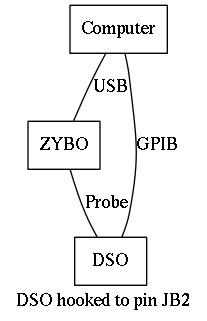
\includegraphics[width=50mm]{block-diagram.png}

\end{frame}

\begin{frame}{Functionality}

  \pause

  \begin{itemize}
  \item User inputs value in C\#
  \item C\# sends value to the ZYBO
  \end{itemize}

  \pause

  \begin{itemize}
  \item ZYBO uses this value as the sleep time
  \item ZYBO starts private timer, sets JB2 high, and sleeps
  \item DSO collects its data
  \end{itemize}

  \pause

  \begin{itemize}
  \item Once finished, the ZYBO sends sleep value to C\#
  \item C\# reads all data off the DSO
  \item C\# finds all data that is high
  \end{itemize}

\end{frame}

\begin{frame}{Tests}

  20 Total Tests
  \begin{itemize}
  \item 10 tests per function
  \item Values per test range from low to high
  \item 10 data points per test
  \item Private timer and DSO data is collected simultaneously
  \end{itemize}

\end{frame}

\begin{frame}{sleep Data for Private Timer}
  \begin{center}
    \begin{tabular}{lrrr}
      Time & Average Measured & Standard Deviation & Percent Error\\
      \hline
      1 & 1 & 1.542\,E-08 & 4.471\,E-05\\
      2 & 2 & 1.369\,E-08 & 2.005\,E-05\\
      3 & 3 & 1.707\,E-08 & 1.476\,E-05\\
      5 & 5 & 1.897\,E-08 & 8.818\,E-06\\
      7 & 7 & 2.088\,E-08 & 5.960\,E-06\\
      10 & 10 & 1.257\,E-08 & 4.575\,E-06\\
      13 & 13 & 1.537\,E-08 & 3.207\,E-06\\
      20 & 13.22 & 0 & -33.92\\
      30 & 13.22 & 0 & -55.95\\
      40 & 13.22 & 0 & -66.962\\
      \hline
    \end{tabular}
  \end{center}
  \small\emph{Note: Time, Average Measured, and Standard Deviation are in seconds}

\end{frame}

\begin{frame}{sleep Data for DSO}

  \begin{center}
    \begin{tabular}{lrrr}
      Time & Average Measured & Standard Deviation & Percent Error\\
      \hline
      1 & 0.989 & 1.17\,E-16 & -0.01\\
      2 & 1.98 & 0 & -1\\
      3 & 2.971 & 2.846\,E-02 & -0.9667\\
      5 & 4.95 & 9.362\,E-16 & -1\\
      7 & 6.96 & 2.108\,E-02 & -0.5714\\
      10 & 9.9 & 1.872\,E-15 & -1\\
      13 & 12.95 & 0 & -0.3846\\
      20 & 19.8 & 3.745\,E-15 & -1\\
      30 & 29.8 & 3.745\,E-15 & -0.6667\\
      40 & 39.8 & 7.49\,E-15 & -0.5\\
      \hline
    \end{tabular}
  \end{center}
  \small\emph{Note: Time, Average Measured, and Standard Deviation are in seconds}

\end{frame}

\begin{frame}{usleep Data for Private Timer}
  \begin{center}
    \begin{tabular}{lrrr}
      Time & Average Measured & Standard Deviation & Percent Error\\
      \hline
      1u & 1.405\,E-06 & 1.452\,E-08 & 40.46\\
      5u & 5.394\,E-06 & 6.454\,E-09 & 7.889\\
      10u & 1.043\,E-05 & 3.163\,E-08 & 4.28\\
      15u & 1.547\,E-05 & 1.038\,E-08 & 3.128\\
      20u & 2.043\,E-05 & 3.773\,E-08 & 2.166\\
      100u & 1.004\,E-04 & 1.88\,E-08 & 0.4358\\
      1m & 1\,E-03 & 1.263\,E-08 & 4.252\,E-02\\
      1.25m & 1.25\,E-03 & 2.211\,E-08 & 3.621\,E-02\\
      10m & 1\,E-02 & 1.175\,E-08 & 4.286\,E-03\\
      100m & .1 & 1.869\,E-08 & 4.514\,E-04\\
      \hline
    \end{tabular}
  \end{center}
  \small\emph{Note: Time, Average Measured, and Standard Deviation are in seconds}
\end{frame}

\begin{frame}{usleep Data for DSO}
  \begin{center}
    \begin{tabular}{lrrr}
      Time & Average Measured & Standard Deviation & Percent Error\\
      \hline
      1u & 1.444\,E-06 & 8.433\,E-09 & 44.4\\
      5u & 5.44\,E-06 & 2.108\,E-08 & 8.8\\
      10u & 1.05\,E-05 & 6.667\,E-08 & 5\\
      15u & 1.551\,E-05 & 3.162\,E-08 & 3.4\\
      20u & 2.044\,E-05 & 1.265\,E-07 & 2.2\\
      100u & 1.005\,E-04 & 5.27\,E-07 & 0.5\\
      1m & 1.001\,E-03 & 3.162\,E-06 & 0.1\\
      1.25m & 1.252\,E-03 & 1.033\,E-05 & 0.16\\
      10m & 1\,E-02 & 1.829\,E-18 & 0\\
      100m & 9.36\,E-02 & 5.164\,E-04 & -6.4\\
      \hline
    \end{tabular}
  \end{center}
  \small\emph{Note: Time, Average Measured, and Standard Deviation are in seconds}
\end{frame}

\begin{frame}{Conclusion}
  \begin{center}
    \begin{tabular}{lrr}
      & SD Private Timer & SD DSO\\
      \hline
      Max & 3.773\,E-08 & 2.846\,E-02\\
      Min & 6.454\,E-09 & 0\\
      Average & 1.757\,E-08 & 2.504\,E-03\\
      \hline
    \end{tabular}
  \end{center}

  \begin{center}
    \begin{tabular}{lrr}
      & Error Private Timer & Error DSO\\
      \hline
      Max & 40.46 & 44.4\\
      Min & 3.207\,E-06 & 0\\
      Average & 3.438 & 2.504\\
      \hline
    \end{tabular}
  \end{center}
  \center\small\emph{Note: Standard Deviations are in seconds}

\end{frame}

\begin{frame}{Conclusion}

  \begin{itemize}

  \item Delay from Private Timer: about 43.21ns on average

  \item Delay from DSO: about 45.27ms on average

  \end{itemize}

  \pause

  \centering
  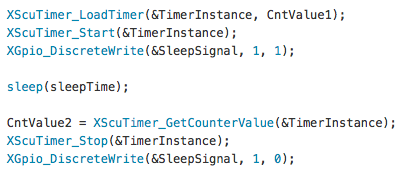
\includegraphics[width=100mm]{code.png}


\end{frame}

\begin{frame}



\end{frame}

\end{document}
